\documentclass[AutoFakeBold,a4paper]{ctexart}
\usepackage{graphicx}
\usepackage{titlesec}
\usepackage{ctex}
\usepackage{xeCJK}
\usepackage{fontspec}
\usepackage{amsmath}
\usepackage{array}
\usepackage{listings}
\usepackage{color, xcolor}
\usepackage{caption}
\usepackage{float}
\usepackage{amsthm,txfonts}
\usepackage{amssymb}
%\usepackage{euler}
\usepackage{fancyhdr}
\usepackage[colorlinks,linkcolor=magenta,citecolor=magenta]{hyperref}
\usepackage{multicol}
\usepackage{titletoc}
\usepackage[biblabel]{cite}
\usepackage[left=1.25in,right=1.25in,top=1in,bottom=1in]{geometry}

\renewcommand\lstlistingname{代码}
%\setCJKmainfont{微软雅黑}[BoldFont=SimHei, ItalicFont=KaiTi]

\pagestyle{fancy}

\fancyhead[RO, RE]{\thepage}
\fancyhead[LO, LE]{\kaishu \leftmark}
\fancyhead[CO, CE]{}

\fancyfoot[RO, RE]{}%lhy1210302421@mail.ustc.edu.cn}
\fancyfoot[LO, LE]{{\kaishu \today}}
\fancyfoot[CO, CE]{}

\setmainfont[Ligatures=TeX]{CMU Serif}
\setsansfont[Ligatures=TeX]{CMU Sans Serif}
\setmonofont[Mapping=]{CMU Typewriter Text}

\setCJKmainfont{PingFangSC-Regular}[BoldFont=PingFangSC-Medium]

\renewcommand{\headrulewidth}{0.1mm} 
\renewcommand{\footrulewidth}{0.1mm}

\lstset{
    basicstyle          =   \sffamily,          % 基本代码风格
    keywordstyle        =   \bfseries,          % 关键字风格
    commentstyle        =   \rmfamily\itshape,  % 注释的风格,斜体
    stringstyle         =   \ttfamily,  % 字符串风格
    flexiblecolumns,                % 别问为什么,加上这个
    numbers             =   left,   % 行号的位置在左边
    showspaces          =   false,  % 是否显示空格,显示了有点乱,所以不现实了
    numberstyle         =   \zihao{-5}\ttfamily,    % 行号的样式,小五号,tt等宽字体
    showstringspaces    =   false,
    captionpos          =   t,      % 这段代码的名字所呈现的位置,t指的是top上面
    frame               =   lrtb,   % 显示边框
    captionpos          =   b       % caption的位置(填t在上,填b在底部)
}

\lstdefinestyle{Python}{
    language        =   Python, % 语言选Python
    basicstyle      =   \zihao{-5}\ttfamily,
    numberstyle     =   \zihao{-5}\ttfamily,
    keywordstyle    =   \color{blue},
    keywordstyle    =   [2] \color{teal},
    stringstyle     =   \color{magenta},
    commentstyle    =   \color[rgb]{0.416,0.6,0.3333}\ttfamily,
    breaklines      =   true,   % 自动换行,建议不要写太长的行
    columns         =   fixed,  % 如果不加这一句,字间距就不固定,很丑,必须加
    basewidth       =   0.5em,
}

\lstdefinestyle{C}{
    language        =   C, % 语言选Python
    basicstyle      =   \zihao{-5}\ttfamily,
    numberstyle     =   \zihao{-5}\ttfamily,
    keywordstyle    =   \color{blue},
    keywordstyle    =   [2] \color{teal},
    stringstyle     =   \color{magenta},
    commentstyle    =   \color[rgb]{0.416,0.6,0.3333}\ttfamily,
    breaklines      =   true,   % 自动换行,建议不要写太长的行
    columns         =   fixed,  % 如果不加这一句,字间距就不固定,很丑,必须加
    basewidth       =   0.5em,
}

\lstdefinestyle{bash}{
    language        =   bash, % 语言选Python
    basicstyle      =   \zihao{-5}\ttfamily,
    numberstyle     =   \zihao{-5}\ttfamily,
    keywordstyle    =   \color{blue},
    keywordstyle    =   [2] \color{teal},
    stringstyle     =   \color{black},
    commentstyle    =   \color[rgb]{0.416,0.6,0.3333}\ttfamily,
    breaklines      =   true,   % 自动换行,建议不要写太长的行
    columns         =   fixed,  % 如果不加这一句,字间距就不固定,很丑,必须加
    basewidth       =   0.5em,
}

% \providecommand{\keywords}[1]{\textbf{\textit{关键字:}} #1}

% \renewcommand{\abstractname}{\textbf{摘要:}}

\begin{document}

\title{\textbf{\Huge 大作业-结题报告}}

\author{陈思睿 \quad 梁恒宇 \quad 吕泓涛 \quad 汤力宇\\
中国科学技术大学 \quad 安徽合肥}

\date{\today}

\maketitle

\ctexset { section = { format={\Large \bfseries} } }
\ctexset { subsection = { format={\large \bfseries} } }

\titlecontents{section}[2em]{\addvspace{1.3mm}\bf}{%
\contentslabel{2.0em}}{}{\titlerule*[5pt]{$\cdot$}\contentspage}

\titlecontents{subsection}[4.2em]{}{\contentslabel{2.5em}}{}{%
\titlerule*[5pt]{$\cdot$}\contentspage}

\titlecontents{subsubsection}[7.2em]{}{\contentslabel{3.3em}}{}{%
\titlerule*[5pt]{$\cdot$}\contentspage}

\pagenumbering{roman}
\tableofcontents

\pagenumbering{arabic}
\setcounter{page}{1}

% \section{小组成员}

% \begin{itemize}
%     \item 陈思睿
%     \item 梁恒宇
%     \item 吕泓涛
%     \item 汤力宇
% \end{itemize}


\section{简介}
沙盒程序是用来保护计算机系统,防止潜在的恶意进程成功实施攻击的一类计算机应用。

当前现有的沙盒程序主要包括内核内置的沙盒工具与用户态沙盒程序两大类,
两种实现方式都存在着较大的缺点。内核沙盒工具有着难以开发、难以调试、
难以提供用户的自由性的问题。用户态沙盒程序则难以逃避多次系统调用带来的性能损耗。

本项目提出一种新的沙盒实现结构,使沙盒程序的结构横跨内核态与用户态,
在精简沙盒结构的同时提高了沙盒程序的自由度,降低了沙盒程序的开发难度,
并且实现了接近原生的沙盒性能。

\section{项目背景}

\subsection{linux由内核提供的沙盒工具}
\begin{itemize}
    \item \textbf{seccomp}\\
    \href{https://en.wikipedia.org/wiki/Seccomp}{seccomp}介绍。
    传统seccomp可以让某个进程进入安全模式,并且阻止其调用所有除了exit(),
    sigreturn(),read(),write()外的所有对file descriptor (FD) 的调用,
    一旦发现此类调用就立即kill进程。后来引入bpf后形成了seccomp/bpf,可以更灵活的设置拦截的规则。
    seccomp使用的是cBPF\cite{calavera2019linux},
    seccomp/bpf以bpf程序的形式定义了一个系统调用的白名单,
    被seccomp/bpf约束的进程可以自由的请求白名单内的系统调用,
    但一旦进程发出了不许可的指令,它将会被立刻终结。
    这种沙盒工具只是利用BPF限制了系统调用,沙盒内外的程序运行环境没有其他区别。
    \cite{2020SandboxLinux}

    \item \textbf{Cgroups}\\
    \href{https://en.wikipedia.org/wiki/Cgroups}{Cgroups}介绍。
    其主要支持四个功能:
    \begin{enumerate}
        \item 限制某些groups的资源使用量(包括CPU,IO,内存等)
        \item 调整优先级,使某些group可以分配到更多的资源
        \item 记录某些group的资源使用量
        \item 控制某些group的运行,具体的可以冻结,快照,重启。
    \end{enumerate}

    \item \textbf{Linux Namespace}\\
    Linux的Namespace机制是一种资源隔离方案。它将 Linux 的全局资源,
    划分为 namespace 范围内的资源,而且不同 namespace 间的资源彼此透明,
    不同 namespace 里的进程无法感知到其它 namespace 里面的进程和资源。
    但是namespace机制有缺陷。
    \begin{enumerate}
        % \item Non-namespace-aware system call interface facilitates
        % the adversary to compromise applications running in containers 
        % and further exploit kernel vulnerabilities to elevate privileges, 
        % bypass access control policy enforcement, 
        % and escape isolation mechanisms.
        \item Non-namespace-aware system调用接口可帮助对手破坏容器中运行的应用程序,
        并进一步利用内核漏洞来提升权限,绕过访问控制策略并逃过隔离机制。\cite{2019Practical}
        \item 某种沙盒使用的安全方案\cite{2019Practical}:
        用自动测试锁定一个container中程序的系统调用。
        然后在实际运行中阻止非锁定的任何系统调用。但是锁定系统调用不算特别理想。
        程序调用的是API,间接执行系统调用,不容易直接发现。
        有的程序将近一半的可能系统调用都没被发掘。对于开发者来说,
        可以加入自己的测试过程来辅助锁定。
    \end{enumerate}

\end{itemize}

\subsection{gVisor为例的用户态沙盒分析}
gVisor 是一款新型沙箱解决方案,其能够为容器提供安全的隔离措施,
同时继续保持远优于虚拟机的轻量化特性。gVisor能够与Docker及Kubernetes实现集成,
从而在生产环境中更轻松地建立起沙箱化容器系统。

gVisor能够在保证轻量化优势的同时,提供与虚拟机类似的隔离效果。
gVisor的核心为一套运行非特权普通进程的内核,且支持大多数Linux系统调用。
该内核使用Go编写,这主要是考虑到Go语言拥有良好的内存管理机制与类型安全性。
与在虚拟机当中一样,gVisor沙箱中运行的应用程序也将获得自己的内核与一组虚拟设备
——这一点与主机及其它沙箱方案有所区别。(gVisor主页)

\textbf{gVisor的结构与问题}

论文\cite{234857}提出来了如下观点:

\begin{enumerate}
    \item 传统来说,hyperviser模式的虚拟化容器有着更好的安全性,
    但是难以保证性能。hostOS结构的容器(如docker)
    的性能更好是由于其运行的若干的虚拟机通过一个统一的完善的通用OS来调度各类资源。
    但是由于hostOS结构中hostOS本身没有运行在容器中,
    其本身的内核bug容易成为被攻击的目标。 
    (详细分析见此文\href{https://opensource.com/business/14/7/docker-security-selinux}
    {Are Docker containers really secure?}\cite{DanielJDocker}) 
    
    \item gviser的存在一些性能问题,如打开关闭文件比传统容器慢了216倍,
    其他操作也普遍慢了很多(2倍到11倍)。
    \item gVisor支持OCI(Open Container Initiative),
    因此docker用户可以自己配置使用默认引擎,runc或者gvisor作为runtime engine。
    \item gVisor结构如下 guestApp-Sentry( VMM+guestOS(linux) )-hostOS,
    多层结构确保程序难以同时攻克每一层的安全缺陷,损害hostOS的安全。
    sentry提供两种工作模式,第一种模式中其追踪并且翻译gusetAPP的系统调用,
    第二种模式中其更像是虚拟机中工作的guestOS,直接服务guestAPP。
    \item gVisor为guestAPP提供了211个syscall(标准linux提供了319种),
    gVisor只需要向hostOS请求55种syscall,
    这些syscall的种类都是通过seccomp技术限制和约束的,
    当sentry被guestAPP劫持并且申请了超出允许范围的syscall时,
    seccomp过滤器会把gVisor杀死从而确保hostOS的安全。
    诸如OPEN和SOCKET这样的操作被设计者认为是极端危险的,
    因此没有被列入许可的syscall,这两个功能是通过复杂的结构设计出来的,
    从而保证可以在不调用hostOS的对应syscall的前提下安全的为guestAPP提供服务。
    这就是为什么gVisor的文件性能如此差。
    \item gVisor对文件服务的实现:
    \begin{itemize}
        \item sentry实现了若干个不同的内置文件系统来尽可能满足guestAPP的请求。
        \item 当有必要读取hostOS文件系统时,他调用Gofer来替其进行文件访问,
        访问结果(文件句柄)通过一个P9 Channel返回给sentry(进程间通讯),
        
        \item sentry得到句柄后需要进行用户态到内核态的转化和上下文切换才能进行读取。
    \end{itemize}
    此过程导致了gvisor在文件访问效率上的低速,但带来了可靠的安全性。
    
    \item 本文提出了若干种对此类容器进行性能测试的方法。
    %\item 其他进程如何实现劫持沙盒管理程序的权限(如open函数),或许能体现BPF的优势,
    % 需要调研现有安全漏洞的形式。
\end{enumerate}

\subsection{恶意进程}

\subsubsection{linux下的恶意进程}

Linux环境下的经典病毒种类有:\cite{LinuxVirus2020}

\begin{itemize}
    \item BillGates 基于僵尸网络的DDOS攻击
    \item DDG 蠕虫式挖矿
    \item SystemdMiner 蠕虫式挖矿
    \item StartMiner 蠕虫式挖矿
    \item WatchdogsMiner 蠕虫式挖矿
    \item XorDDos 基于僵尸网络的DDOS攻击
    \item RainbowMiner 蠕虫式挖矿
\end{itemize}


\subsubsection{经典攻击方法}

在这几篇文章\cite{di2015elf} \cite{rieck2008learning}中介绍了几种经典的恶意进程攻击手段:

\begin{itemize}
    \item 操作系统中的一个用户态组件——动态装载器,
    负责装载二进制文件以及它们依赖的库文件到内存中。
    二进制文件使用动态装载器来支持导入符号的解析功能。有趣的是,
    这恰好就是一个面对加固应用的攻击者通过泄漏库地址与内容尝试“重塑”一个符号的表现。
    windows下的svchost.exe攻击或者linux下的elf攻击都是利用了这个组件进行的攻击。
    \item 早期的栈溢出利用依赖于向缓冲区中注入二进制代码(称为shellcode)的能力,
    并需要覆盖在栈上的一个返回地址使其指向这个缓冲区。随后,当程序从当前函数返回时,
    执行流就会被重定向到攻击者的shellcode,接着攻击者就能取得程序的控制权。
    
\end{itemize}

\subsubsection{恶意进程行为}

卡巴斯基安全实验室在对一个新型zeus变种木马的报告中给出了如下的分析:\cite{ZeuS2018}

\begin{itemize}
    \item 此木马功能非常丰富,包括使用VNC远程桌面控制电脑,截屏并发送,
    读取本地数据并发送,读取用户所有操作并发送,通过注册表开机自动启动,
    监测是否处于沙盒环境并且在沙盒中自动停止活动,监测注册表以防止自己的自动启动被清除。

    \item 此木马的传播主要通过邮件,在恶意邮件中包含一个doc文件作为附件,
    打开后office会提示需要启用宏来查看完整信息,
    一旦用户点击启用宏后,此木马会自动解码并且将自己复制进svchost.exe
    ,然后其遍可以开始运行各种功能,包括剩余模块的下载,劫持浏览器,窃取本地数据等。
    
    \item 此木马通过读取进程列表以判断是否有正在打开的浏览器,
    然后当存在浏览器的时其会通过浏览器的安全漏洞劫持网页,
    修改用户正在访问的银行网页,截取其输入的密码、账号、pin、等内容并且发送给服务器。
    
    \item 此木马对沙盒有有特殊的监测机制,
    运行在沙盒内的时候系统中会出现若干特征性的监控类设备驱动,
    当发现自己运行在沙盒中时,木马将停止活动以防止自己被安全人员监测出来。
\end{itemize}

\subsubsection{小结}

此分析给我们带来了如下的提示:
\begin{itemize}
    \item 针对某个具体的漏洞来设计沙盒是不切实际的,随着系统体量的膨胀,
    漏洞的存在是不可避免的,至今linux和windows也无法完全杜绝对系统代码的恶意篡改。
    \item 各类资源的隔离对于沙盒的安全性至关重要,必须确保沙盒内的进程只能访问有限的文件服务或者系统服务。
    \item 任何需要与被隔离进程直接交互的服务都有被污染的可能,
    因此多层的隔离或者使用类似于BPF的无法污染的实现方式可以有效的提高对恶意进程的控制力度。
\end{itemize}


\subsection{docker安全}
下面是docker安全性的具体实现方式\cite{boettiger2015introduction} \cite{rad2017introduction}

\begin{enumerate}
    \item 通过namespace,不同docker容器无法访问其他的进程,
    在容器位置向系统请求进程列表会只能看到少数几个局部的容器内进程,无法发现主机的其他进程。
    通过这种技术,类似于zeus的劫持浏览器进程的木马难以危害主机安全。
    
    \item 通过namespace,每个docker会被置入隔离的网络环境中,
    对外的网络功能是通过在每个docker上运行虚拟的网卡并且以桥接模式(默认)与主机网卡链接来实现的。
    在这种情况下可以通过网络安全策略的方式直接控制容器进程的非法网络访问。\\
    \textbf{libnetwork}:docker的网络功能实现的具体技术
    
    \item 利用libcontainer(以及namespace)来实现了对文件系统的保护,
    libcontainer中的chroot技术可以限制某个子系统对应的根目录(rootFS),
    即在容器内的进程来看,当前FS的root就是实际所在的子目录,因而其无法读取或访问主机上的其他文件。
    
    \item cgroup(控制组)是用于限制进程对CPU、内存、网络带宽等运行资源的占用强度的,
    其也可以用来限制容器内程序对设备的访问。不同的进程被组合成一个cgroup,
    作为一个整体参与资源的调度,并且可以通过cgroup组策略来限制当前group可以占用多少资源。
    且cgroup可以嵌套,一个cgroup里面可以包含多个子cgroup。
    如整个docker可能被放在一个cgroup中以限制总资源使用量,
    然后docker里面的每个容器中的进程也各自建立cgroup,
    参与划分docekr-group分配到的总的资源。
    
    \item 联合文件系统(Unionfs),实质上概念很简单,
    此文件系统不管理物理存储,只是依赖于某一个通用的文件系统,
    并且把不同文件夹的内容映射到同一个文件目录内。似乎是docker的重要组成部分。
\end{enumerate}

在这篇文章中,分析了docker结构的安全性:\cite{bui2015analysis}

\begin{itemize}
    \item 文章基于的模型如下:当hostOS中运行的docker容器中有一部分被恶意进程完全控制了,
    其可以对系统进行如Denial-of-Service 和 Privilege escalation的攻击。
    \item 为了在这种情况下保护系统安全,容器应当做到如下几点:
    \begin{itemize}
        \item process isolation 进程间的隔离
        \item filesystem isolation  文件系统的隔离
        \item device isolation  设备的隔离
        \item IPC isolation 进程间通讯的隔离
        \item network isolation 网络的隔离
        \item limiting of resources 限制资源的使用量
    \end{itemize}
\end{itemize}

对于路线一(见\ref{路线一})或路线三(见\ref{路线三}),我们可以参考docker的安全策略,
此策略在各个角度上都有较好的安全性,而且性能相当的高。

\subsection{macOS沙盒分析}

\subsubsection{macOS沙盒的权限设置}

macOS沙盒中有如下的权限设置\cite{hoog2011iphone}:

\begin{itemize}
    \item Essentials:是否使用访问控制技术
    \item Network:接收和发送网络数据的权限
    \item Hardware:硬件权限,如照相机
    \item App Data:访问地址簿,位置,日历的权限
    \item File Access:其中设置是否拥有访问系统全部文件的权限已被剥离。
    读写限制十分严格,只有用户主动操作才能实现一般文件的读写
    (通过脱离程序语境的Powerbox机制——一个选择文件的对话框),
    否则只有应用程序自己的目录是可见的。下载内容、图片、音乐、电影各有特殊限制规则。
\end{itemize}

\subsubsection{应用程序沙盒化}

\begin{itemize}
    \item 在使用苹果的开发软件(如Xcode)进行build时启用沙盒并进行沙盒权限确认即可。
    \item 建立于MacOS沙盒不是程序的义务,但却是上架Mac App Store的必要条件。
    就算上架MAS,沙盒机制也是可以绕过去的。开发者在商店之外提供一个程序外挂供用户自由安装。
    由上架MAS的程序指挥外挂进行沙盒外操作即可。
    \item iOS是一个从一开始就彻底应用沙盒机制的系统,
    正常情况下,所有 iOS 设备都只能安装 App Store 中的应用程序,
    而所有这些应用程序都彻底采用了沙盒机制,不能访问除自己目录之外的资源。
    虽然保证了安全性,但是也牺牲了一些便利性,如他们的应用程序无法调用其它程序配合完成任务,
    导致必须重复实现各种已有的功能(如pdf阅读功能)。
\end{itemize}

\subsubsection{沙盒机制}

沙盒机制见下图:

\begin{figure}[H]
    \centering
    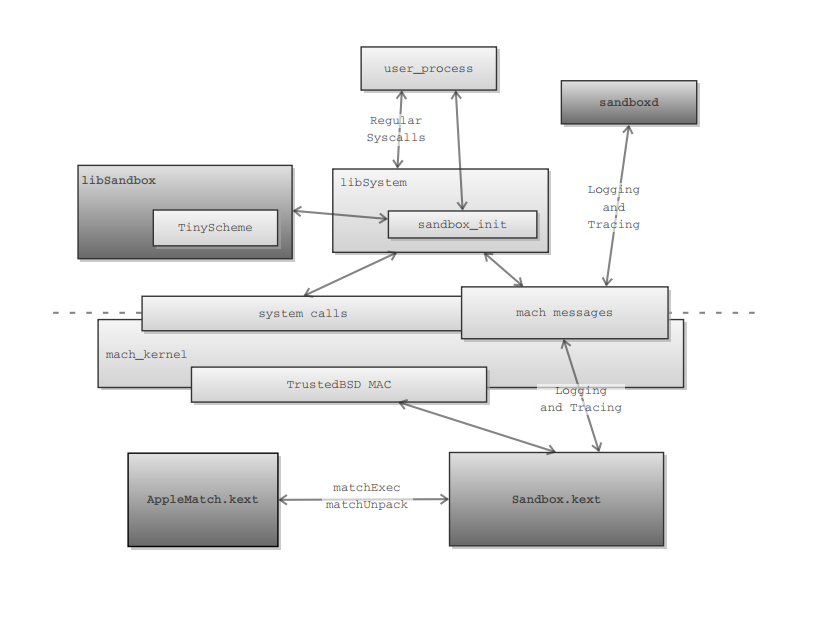
\includegraphics[width=0.92\columnwidth]{../feasibility/Sandbox_Structure.PNG}
\end{figure}

\begin{figure}[H]
    \centering
    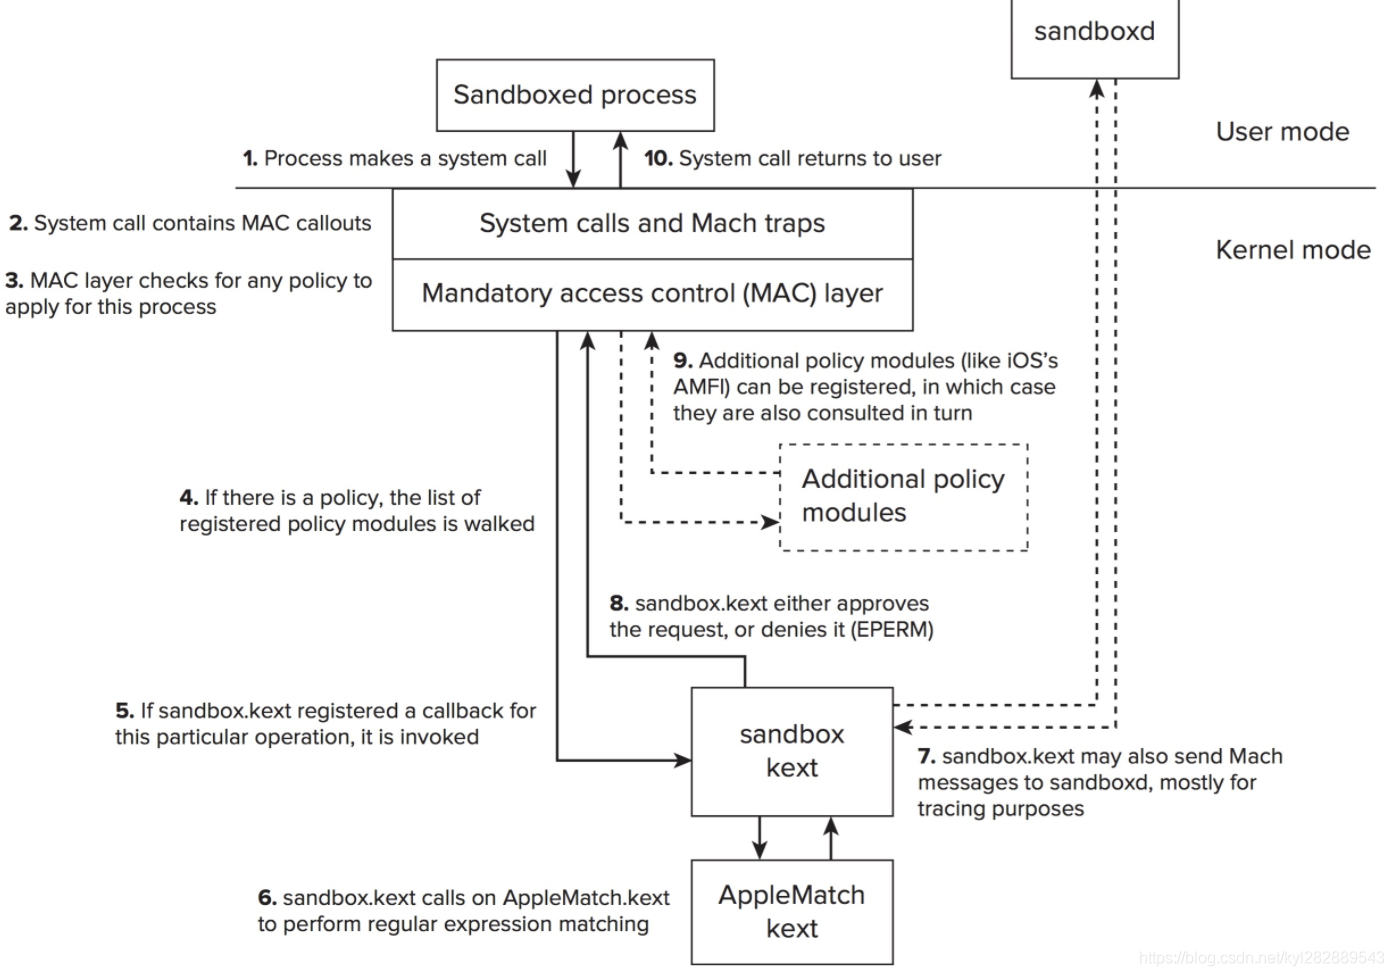
\includegraphics[width=0.92\columnwidth]{../feasibility/Sandbox_Process.png}
    \caption{沙盒机制\cite{blazakis2011apple}}
\end{figure}

\begin{itemize}
    \item 新的应用程序需要经过初始化。原先的、还未运行过的程序没有被sandbox约束,
    但是在初始化过程中,如果动态链接器确认了程序启用sandbox,
    就会根据程序中的权限设置(entitlements)编译出profile。在每次程序运行时,
    动态链接器都会在应用程序的语境中,根据这个profile初始化沙盒,
    然后才把控制权递交给程序。
    \item 流程
    \begin{itemize}
        \item 1 进程尝试进行一次系统调用(system call),调用内核功能。
        \item 2、3 MAC层需要根据该进程的安全策略判断此次系统调用是否可以执行。
        \item 4、5、6、7、8、9 如果存在策略的话,通过sandbox.kext(提供system call的hook函数)和AppleMatch.kext(解析沙盒的profile)两个内核扩展实现权限的检查。
        \item 10 返回调用结果
    \end{itemize}
    \item XPC服务
    \begin{itemize}
        \item 是MacOS下的一种IPC(进程间通信)技术, 它实现了权限隔离, 
        使得App Sandbox更加完备。
        \item 将程序隔离成多块能提高稳定性,在某部分crash时,主程序依然运作。
        \item 沙盒中应用无法让子进程拥有比自身更高的权限,但是开发者可以设定XPC helpers,
        它们各自运行在自己的沙盒中并拥有刚好供功能实现所需的权限。实现权限分割,
        安全性就进一步提高了。
    \end{itemize}
    \item 和linux下的seccomp有相似之处,即在内核中对system call进行过滤。
    沙盒初始化就像seccomp程序启用。
\end{itemize}

\subsubsection{macOS沙盒优缺点}

\begin{itemize}
    \item \textbf{优点}
    \begin{enumerate}
        \item 安全性高。不影响性能。
        \item 开发者使用方便。
        \item 对于用户需求的敏感访问有系统接管办法,如Powerbox。
    \end{enumerate}
    \item \textbf{缺点}
    \begin{enumerate}
        \item 自由度低。非MAS平台的应用,大部分没有采用Sandbox机制。
        \item 沙盒有不可避免的漏洞:
        \begin{itemize}
            \item 沙盒在应用程序的语境下初始化,
            如果程序偶然在沙盒初始化完成前就运行了代码,就存在保护失效的可能性。 
            事实上bug确实发生了。\cite{blochberger2019state}
            \item 在规则内做出背离沙箱的行为。\cite{Mojave2018}尽管Apple阻止应用程序注册全局接收分布式通知,
            但没有任何机制能够阻止沙箱应用程序注册接收任何通知。因此,如果按照名称,
            注册所有的分布式通知,恶意应用程序可以轻而易举地避开Apple针对沙箱的限制。
            尽管这需要一些额外的代码来实现,但其带来的影响是造成任何应用程序都可以通过遍历注册,
            来接收(捕获)到所有分布式通知,包括在沙箱中也是如此。
        \end{itemize}
    \end{enumerate}
\end{itemize}

\subsubsection{小结}

Apple系统的安全性很大程度上都无法离开一种强大的闭环生态,想在设备上运行就必须得遵守相应的约定。
而Linux是一个非常开放的环境,就此而言,我们不可能让应用在开发的时候就强制开启沙盒,
所以我们几乎是没有办法实现一个兼顾安全性、性能、通用性的沙盒的。

对macOS沙盒结构的研究,对后续路线一和路线三均有启发。
拦截系统调用是目前大多数沙盒的做法,在Linux下,我们可以借助BPF实现系统调用的拦截。
同时,我们可以用编写安全策略加额外策略模块的方式来认证每次系统调用是否安全,若安全则允许调用,
若不安全则拒绝调用。

\section{项目介绍}

\subsection{项目设计思路}
本项目的设计基于如下观察:用户态的程序编写简单,测试运行简单,
适合用来尝试实践复杂的沙盒逻辑,但是用户态的程序为了实现沙盒的功能,需要操作系统通过复杂操作来传递其所需要的上下文数据,
需要操作系统通过复杂方式进行沙盒程序的回调,这两者都会产生较大的性能开销。更甚至,沙盒程序的功能与内核功能高度重合,因此需要频繁的进行系统调用,
更是会带来很多的上下文切换,产生不必要的性能开销。相对应的,内核中直接实现的沙盒程序则需要通过重新编译整个内核才能测试其在内核正常工作流程中是否能正常工作,
一旦出现错误,更可能会导致整个操作系统发生崩溃,所以只有少数几种高度重要的沙盒工具被内置在了linux内核中,
并且也少有人尝试自己在内核中增加新的沙盒特性来实现某些具体的沙盒保护目的。

而我们的项目基于沙盒程序的现有现状,尝试借鉴用户态沙盒程序的运行流程,但是将进行回调的用户态程序替换成通过模块方式载入到内核代码链接范围的内核态程序段。
由于内核态程序可以原生的调用大部分内核函数ABI,因此在实现沙盒功能的时候有着更好的性能表现,同时上下文的传递也由于同样在内核空间中进行,因此可以直接进行读取。
在这种结构下,沙盒程序可以实现较好的性能,编写沙盒程序也变得与编写用户态程序一样非常简单。

最终的项目结构体现出了“策略与机制相独立”的操作系统设计哲学,我们的项目对内核的修改仅限于20行以内的修改,简单的创建了静态的系统调用劫持点和相对应的程序回调机制。
而实际的回调函数则是在用户态进行独立编译后,使用内核模块动态装载机制,临时的载入到内核空间中进行运行,产生沙盒的隔离功能。

\subsection{整体结构}
本项目整体分为三个部分:第一部分为可装载到内核中的内核模块,其中包装了实现了沙盒逻辑功能的一系列回调函数和服务回调函数和沙盒功能持久化的一系列数据结构。
第二部分通过修改内核源码实现,用来调用模块中实现的回调函数,将沙盒程序加入到内核正常的工作流程中。第三部分是用户态的装载器,
其负责将被隔离程序作为子进程调用,并且自动完成沙盒模块的装载工作,将子进程纳入cgroup的监测范围内,之后其等待其子进程运行结束,
并且在运行结束后自动把装载进去的模块卸载出来,还原其对操作系统的影响。

\subsection{可载入模块}
本项目共实现了三个不同的模块,实现了三种不同的沙盒隔离逻辑。
\begin{itemize}
    \item {\ttfamily sBPF\_redir}:这个模式的sBPF程序会将被隔离程序的所有文件访问路径替换到一个指定的由沙盒程序维护的路径中,
    阻止对原始文件目录的所有文件访问请求,全部通过篡改访问操作传入参数的方式重定向到沙盒目录中。
    \item {\ttfamily sBPF\_cow}:这个模式的sBPF程序会允许程序对原文件系统的文件读取请求,便于运行大部分通用的程序,但是一旦出现写操作的文件请求,
    会在沙盒目录中复制一份对应的文件,并且把从此以后对同一个文件的所有读写操作全部重定位到沙盒目录中的备份中。
    通过这种模式,可以在保证程序正常运行的条件下,保护原文件系统的文件内容不被修改,保护用户数据安全。
    \item {\ttfamily sBPF\_permission}: 这个模式的sBPF沙盒运行用户指定一个文件目录,则会限制被隔离程序的所有文件请求不能超出此文件目录和其子目录的范围。
    linux的文件权限管理只能限制在某个用户文件夹层次上,而这个模式让用户可以给被隔离程序建立一个工作目录,使其文件访问不得超出此目录范围,
    从而保护用户其他数据的安全。
\end{itemize}


\subsection{内核的修改}
内核的修改较为简单,主要是添加了标志了是否载入了沙盒程序的标志位,以及添加了调用沙盒程序的调用入口,通过函数指针就可以简单的实现出来。
通过export宏定义使其可以被载入的模块读取和修改,就完成了所有的内核修改。

\subsection{loader}
loader是我们实现的一个简单的前端,自动化的完成调用目标程序,装载和卸载sbpf模块的,简化了沙盒的使用体验。其还附加了与cgroup等内核态程序通讯的功能,
增强了沙盒的整体功能性。

\section{项目实施过程的记录}
\subsection{BPF的相关尝试}
本项目最初计划通过使用bpf程序的形式来实现沙盒的运行逻辑,此bpf程序的功能与当前结构中的沙盒内核模块相同,
这是考虑到bpf程序可以直接通过检查寄存器组的方式获取到系统调用的传入参数和相关上下文,并且有着更为严谨的安全策略保证其安全性。
(bpf相关的基本概念可以参考前几次报告的内容,由于最终实现方式中没有使用bpf结构,于是没有这本文中涉及)但是经过了大量的调研与实践,
我们最终没能成功的实现基于bpf的安全沙盒,这也导致我们大量的工作白费,导致了最终成品中没能实现太多更加复杂可靠的安全策略,
而只是作为技术demo性质,实现了一些较为简单的安全特性。我们的bpf模式沙盒实质上已经完成了系统调用的侦测和系统调用上下文的获取,
但是却在将沙盒程序的运行结果传回到原始运行流的过程中遇到了无法解决的困难。这是linux环境下可以编译bpf程序的两个主流编译器各自存在不同的问题,
原先使用的直接从C进行bpf编译的程序在编译kprobe程序进行系统调用侦听时,由于其使用的ABI不正确(我们尝试了若干个不同的kernel版本,都不成功),
总是不能稳定的获取到正确的上下文。而更加高级的bcc编译工具组则不知为何,没有支持我们需要使用的一个将数据直接写入用户态内存的bpf\_helper函数,
这导致我们完全无法编译出原先设计的bpf沙盒程序,而程序本身又过于复杂,几乎没办法直接用汇编方式实现,于是最终只能放弃了使用bpf实现的计划。
作为替代,我们便使用了内核模块的方式来进行加载。内核模块的运行原理与bpf程序几乎相同,并且可以更加简单的直接通过静态调用点来执行调用,
在工期告急的情况下变成了我们的唯一选择。

\subsection{内核模块方式的实现}
基于我们对BPF内核源代码的部分研究,现在我们设计了一种与BPF的思想类似,都能支持一种灵活的调整内核态程序的功能的方式。
这种方式通过修改内核+使用内核模块来实现。

在确定使用内核模块来实现本项目后,我们就开始着手对内核进行修改。虽然内核修改的代码量非常少,但是由于对linux的源码编程体系不熟悉,
我们通过了大量的努力才成功的编译出了第一版可以正确进行回调的内核。每次修改内核都要经历长达十几分钟的内核编译过程,
并且每次替换内核都有导致系统崩溃的可能,于是这个阶段给我们带来的巨大的痛苦。  

在内核修改完成后,后续的工作就变得简单了许多,只要不断的编写出不同的测试模块和测试程序,并且将他们组合起来进行多项测试,就完成整体的内核态的工作。
而用户态的loader则是经过一段时间的调试后,就可以顺利的和内核模块配合进行工作了。

\section{功能演示与性能测试}
\subsection{功能演示}
这个功能演示演示的是使用cow模式隔离一个测试程序,这个测试程序会尝试读取原始文件系统中本来存在的一个文件并且打印其内容,
之后会尝试篡改统一个文件的内容,然后其会再进行一次读取和打印。 可以看到这个程序的两次读取都成功了,运行的效果与其正常运行相同,然而原始文件并没有被修改,
而是在沙盒目录中创建了另一个文件并且修改了这个文件。

\begin{figure}[H]
    \centering
    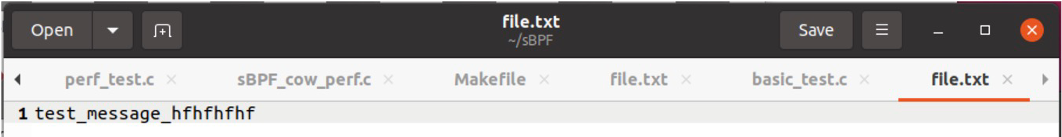
\includegraphics[width=\columnwidth]{pic8.png}
    \caption{初始文件}
\end{figure}

首先,将一个初始文件放置在{\ttfamily \~{}/sBPF/file.txt},文件的内容如上图所示。

\begin{figure}[H]
    \centering
    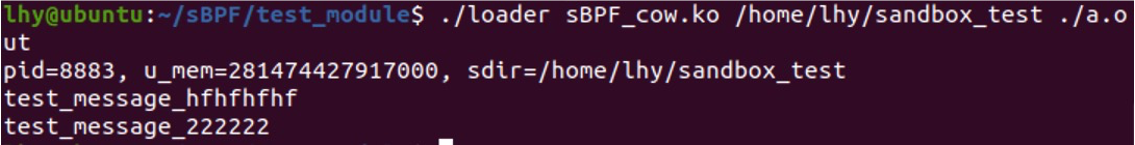
\includegraphics[width=\columnwidth]{pic6.png}
    \caption{将沙盒载入内核}
\end{figure}

然后,将沙盒载入内核,沙盒管控一个程序,该程序会对该文件进行一次读取、写入、读取操作,写入的内容为
{\ttfamily test\_message\_222222}。

\begin{figure}[H]
    \centering
    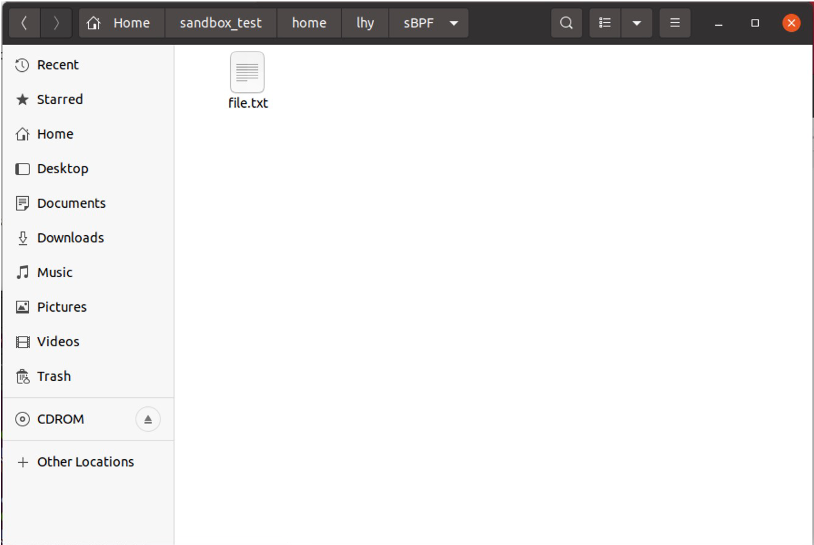
\includegraphics[width=\columnwidth]{pic7.png}
    \caption{沙盒文件路径}
\end{figure}

程序执行结束后,写入的文件出现在沙盒路径中。

\begin{figure}[H]
    \centering
    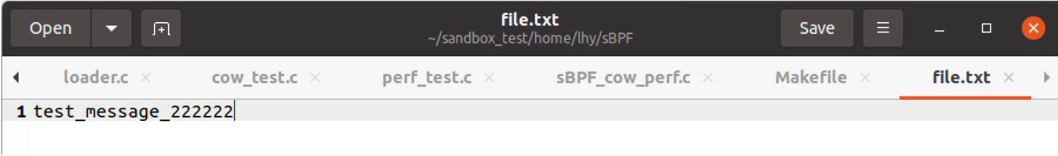
\includegraphics[width=\columnwidth]{pic9.png}
    \caption{沙盒文件内容}
\end{figure}

打开文件,内容是写入的新内容,原文件则依旧位于原先的位置,并且内容没有发生改变。

\subsection{性能测试}
我们对我们的沙盒程序在cow模式下进行了性能测试(这是由于这个模式比较接近正常沙盒系统的运行状况),性能测试的内容是重复百万次文件的打开,读写,关闭。
因为在虚拟机中运行,时间无单位,只进行相对对比。可以看到我们的程序很接近原生的性能,明显好于gVisor的性能\cite{234857}。

\begin{figure}[H]
    \centering
    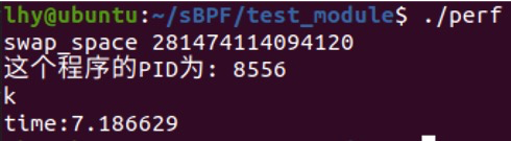
\includegraphics[width=0.49\columnwidth]{pic11.png}
    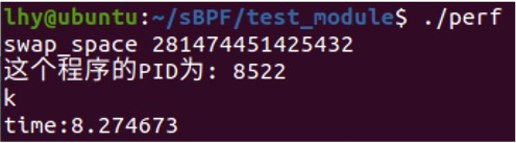
\includegraphics[width=0.49\columnwidth]{pic12.png}
    \caption{正常读写(左图),沙盒读写(右图)}
\end{figure}

\begin{figure}[H]
    \centering
    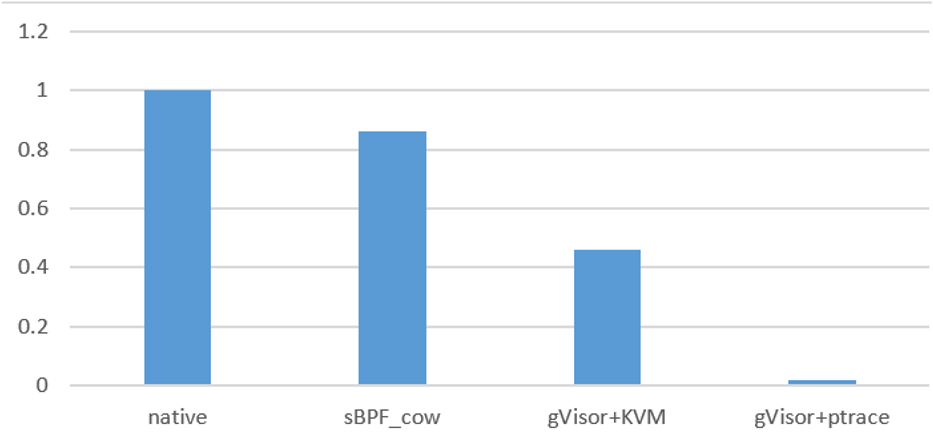
\includegraphics[width=\columnwidth]{pic13.png}
    \caption{效率对比}
\end{figure}

\subsection{项目总结}
本项目在整个过程中历经波折,甚至修改过立项之初的一些想法,最终才达到了今天的完成状态。期间本组的队员们遇到了很多超出想象外的困难,
并且在解决这些困难的过程中增加了我们对linux内核运行过程的很多理解。开学时,我们对操作系统的运行原理一窍不通,
甚至一开始时对内核态用户态的区别都一切不通。通过在内核态进行很多的修改和测试,我们解决很很多诸如内存管理权限问题、
不同用户进程对内存地址的理解不同的问题(由于段页式内存对每个进程进行的内存抽象),在完成了此项目的过程中我们通过查找资料与多种编程尝试,
成功的从理论上和实践上解决了这些问题。在项目的整个推进过程中,我们也实现了成功的分工和时间规划,
高效有序的完成了整个项目的推进,并且最终完成了这个项目。

\bibliography{../paper.bib}
\bibliographystyle{ieeetr}

\end{document}